% file: C01_combined_cache.tex
% author: C. Menges

\documentclass{standalone}
\usepackage{mathtools}
\usepackage{pgfplots}
\usepackage{tikz}
\usetikzlibrary{patterns,arrows, arrows.meta, bending, shapes, 3d, calc, fit, positioning}

% original taken from:
% https://tex.stackexchange.com/questions/154842/using-pattern-inside-tikz-shapes-with-dropped-shadows/155100#155100
\makeatletter
\tikzset{% customization of pattern
	% based on <m.wibrow@gm...> - 2013-03-24 07:20: 
	hatch distance/.store in=\hatchdistance,
	hatch distance=1cm,
	hatch thickness/.store in=\hatchthickness,
	hatch thickness=0.3cm
}
\pgfdeclarepatternformonly[\hatchdistance,\hatchthickness]{north east hatch}% name
{\pgfqpoint{-\hatchdistance}{-\hatchdistance}}% below left
{\pgfqpoint{2\hatchdistance}{2\hatchdistance}}% above right
{\pgfpoint{\hatchdistance-1pt}{\hatchdistance-1pt}}%
{
	\pgfsetcolor{\tikz@pattern@color}
	\pgfsetlinewidth{\hatchthickness}
	\pgfpathmoveto{\pgfqpoint{0pt}{0pt}}
	\pgfpathlineto{\pgfqpoint{\hatchdistance}{\hatchdistance}}
	\pgfusepath{stroke}
}
\makeatother
%%%%%%%%%%%%%%%%%%%%%%%%%%%%%%%%%%%%%%%%

\pgfplotsset{axisConfig/.style=
	{
		ybar stacked, axis on top,
		bar width=1cm,
		x=1cm,
		enlargelimits=0.1,
		ymajorgrids, tick align=inside,
		major grid style={draw=white},
		tickwidth=0pt,
		y axis line style={opacity=0},
		ylabel={\# cells},
		xlabel={indices},
		symbolic x coords={0,1,2,3,4,5,6},
		xtick=data,
		x tick label style={anchor=north},
		ytick distance={1},
		y=1cm,
		label style={font=\large},
		tick label style={font=\large}  
	}
}

\begin{document}
	% t
	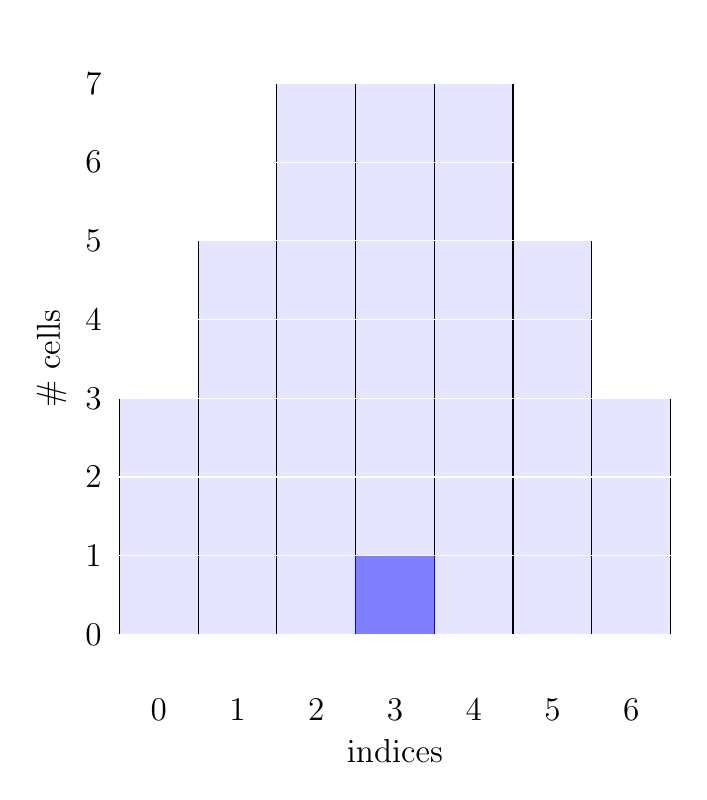
\begin{tikzpicture}[baseline=3cm]
	\begin{axis}[axisConfig]
	% base cell
	\addplot+[ybar, fill=blue!50] plot  coordinates
	{(0,0)(1,0)(2,0)(3,1)(4,0)(5,0)(6,0)};
	
	\addplot+[ybar, black, fill=blue!10] plot  coordinates
	{(0,3)(1,5)(2,7)(3,6)(4,7)(5,5)(6,3)};
	\end{axis}
	\end{tikzpicture}
	
	\begin{huge}
		$\xRightarrow{t \rightarrow t + 1}$
	\end{huge}
	
	% t + 1
	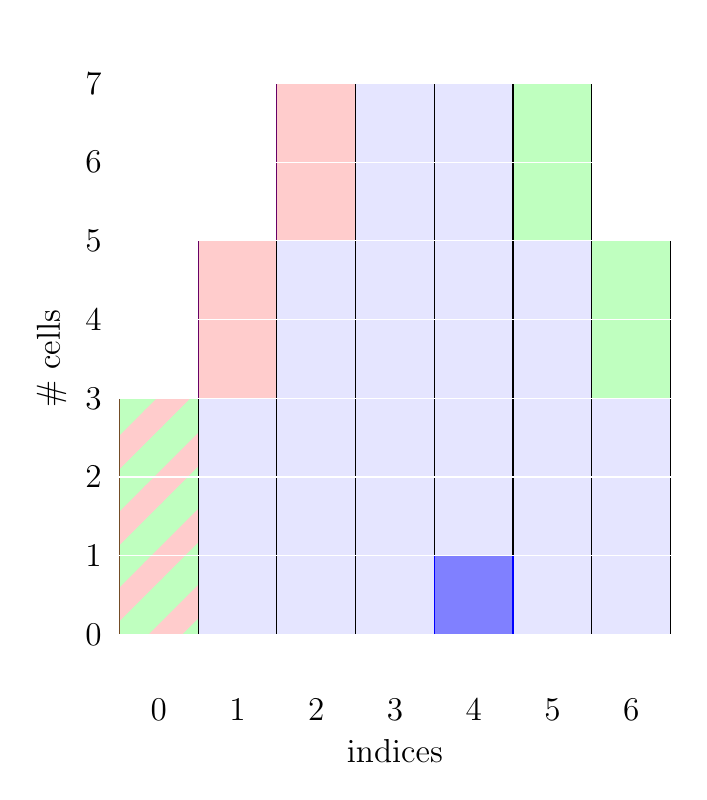
\begin{tikzpicture}[
	baseline=3cm,
	Pattern/.style = {
		pattern=north east hatch,
		pattern color=red!20,
	},
	]
	\begin{axis}[axisConfig]
	% base cell
	\addplot+[ybar, fill=blue!50] plot  coordinates
	{(0,0)(1,0)(2,0)(3,0)(4,1)(5,0)(6,0)};
	
	\addplot+[ybar, black, fill=blue!10] plot coordinates
	{(0,0)(1,3)(2,5)(3,7)(4,6)(5,5)(6,3)};
	
	\addplot+[ybar, preaction={fill=green!25}, Pattern] plot coordinates
	{(0,3)(1,0)(2,0)(3,0)(4,0)(5,0)(6,0)};
	
	% additions
	\addplot+[ybar, fill=green!25] plot coordinates
	{(0,0)(1,0)(2,0)(3,0)(4,0)(5,2)(6,2)};
	
	% deletions
	\addplot+[ybar, fill=red!20] plot coordinates
	{(0,0)(1,2)(2,2)(3,0)(4,0)(5,0)(6,0)};
	
	\end{axis}
	
	\end{tikzpicture}
\end{document}